% Chapter Template

\chapter{PID/PD Control} % Main chapter title

\label{Chapter6} % Change X to a consecutive number; for referencing this chapter elsewhere, use \ref{ChapterX}

\lhead{Chapter 6. \emph{PID/PD Control}} % Change X to a consecutive number; this is for the header on each page - perhaps a shortened title

Among the many methods available for mathematical control of the quad-rotor, a well tuned PID controller offers both relative robustness and a simple mathematical representation. In this chapter we derive and test the PID control scheme for attitude and 3D position control of a quad-rotor.  


\section{Deriving the Control Expressions}

The control of the quadrotor requires three independent PID controllers for the x, y, and z directions. In addition, the attitude stability of the aircraft is accomplished by three independent PD controllers for each of the Euler angles $(\phi,\theta,\psi)$ . It is assumed for the purpose of simulation that the input to the control expressions includes accurate knowledge of the system state. In other words, it is assumed that the process noise and the measurement noise are zero. Given the natural complexity of the system, inclusion of stochastic processes into the model is left for further work. As in \cite{Luukkonen} and \cite{bouabdallah2004pid}, the control algorithm proceeds as follows (Algorithm \ref{alg61}).

\begin{itemize}
\label{alg61}
\item Algorithm 6.1
    \begin{enumerate}
    \item The position control expressions give the 'commanded' linear accelerations that are required to drive the system to the desired state.
    \item Given the commanded linear accelerations, the necessary total thrust, pitch, and roll are determined.
    \item The commanded torques about the three axes of the quad-rotor are given by PD controllers using the commanded yaw, pitch, and roll as angular set points.
    \item Given the commanded total thrust and the commanded torques, the motor speeds can be determined.
    \item Once the motor speeds are known, the system model can be used to obtain the updated state of the system.
    \item Go to step 1.
    \end{enumerate}
\end{itemize}


Our goal in the following derivation is to arrive at expressions for the motor speeds that are required to drive the system to the desired state. 

%$P_e = \left( \begin{array}{c}
%x_e\\y_e\\z_e\\
%\end{array}\right) = error\text{ }in\text{ }position$\\

$P_c = \left( \begin{array}{c}
x_c\\y_c\\z_c\\
\end{array}\right) = desired\text{ } (commanded)\text{ }set\text{ }point\text{ }location $\\

$P = \left( \begin{array}{c}
x\\y\\z\\
\end{array}\right) = actual \text{ }position\text{ }at\text{ }time\text{ }step\text{ }k$\\

The discrete-time PID control expressions are formulated using these vectors.

\begin{equation}
    \label{eq:acc_comm}
    \ddot{P_c} = k_p(P_c - P) + k_i \sum_k (P_c-P) + k_d(\dot{P}_c - \dot{P})  
\end{equation}



%\begin{equation}
% \label{eq:malus}
%  I_\theta = I_0\cos^2\theta
%\end{equation}

%Reference: \eqref{eq:malus}


$\ddot{P_c}$ is the vector of commanded accelerations.

\begin{equation}
    \ddot{P_c} = \left( \begin{array}{c}
    a_x\\a_y\\a_z\\
    \end{array}\right)
\end{equation}

Equation \ref{linforce} can be rearranged to give


\begin{equation}
    \label{eq:acc_from_model}
    \ddot{P_c} = - g e_{inz} + (\frac{1}{m}) (T e_{qrz}) R 
\end{equation}.


$ e_{inz} = \left( \begin{array}{c}
0\\0\\1\\
\end{array}\right) \text{  }$ (in the inertial reference frame)

$ e_{qrz} = \left( \begin{array}{c}
0\\0\\1\\
\end{array}\right) \text{  }$  (in the quad-rotor reference frame)

$\phi$ and $\theta$, and the total thrust $T$ can be determined algebraically, assuming we know $\ddot{P_c}$ and $\psi$.\\

\begin{equation}
    \label{eq:thrustTransformation}
    R^T ( \ddot{P_c} + g e_{inz}) = (\frac{1}{m}) (T e_{qrz})
\end{equation}


\begin{equation}
\begin{split}
    &\left( \begin{array}{ccc}
        c(\psi) c(\theta) & s(\psi) c(\theta) & -s(\theta)\\
        c(\psi) s(\theta) s(\phi) - s(\psi) c(\phi) & s(\psi) s(\theta) s(\phi) + c(\psi) c(\phi) & c(\theta) s(\phi)\\
        c(\psi) s(\theta) c(\phi) + s(\psi) s(\phi) & s(\psi) s(\theta) c(\phi) - c(\psi) s(\phi) & c(\theta) c(\phi)\\
    \end{array} \right)\left( \begin{array}{c} a_x\\a_y\\a_z+g\\\end{array} \right)\\
    &= \frac{1}{m} \left( \begin{array}{c} 0\\0\\T\\ \end{array} \right) 
\end{split}
\end{equation}

The matrix equation above is then written as three independent scalar expressions.

%\begin{equation}
%\begin{split}
%first part &= second part 1 \\
%           &= second part 2
%\end{split}
%\end{equation}



\begin{equation}
    \label{eq:matrixeqline1}
    a_x c(\psi) c(\theta) + a_y s(\psi) c(\theta) - s(\theta)( a_z + g ) = 0
\end{equation}

\begin{equation}
    \label{eq:matrixeqline2}
    \begin{split}
    & a_x (c(\psi) s(\theta) s(\phi) - s(\psi) c(\phi))\\ 
    &+ a_y (s(\psi) s(\theta) s(\phi) + c(\psi) c(\phi))\\ 
    &+ ( a_z + g )c(\theta) s(\phi) = 0
\end{split}    
\end{equation}

\begin{equation}
    \label{eq:matrixeqline3}
    \begin{split}    
    & a_x (c(\psi) s(\theta) c(\phi) + s(\psi) s(\phi))\\ 
    &+ a_y (s(\psi) s(\theta) c(\phi) - c(\psi) s(\phi))\\ 
    &+ ( a_z + g )c(\theta) c(\phi) = (\frac{T}{m})
\end{split}
\end{equation}


Next, we divide Equation \eqref{eq:matrixeqline1} by $c(\theta)$ and solve for $\theta$.

\begin{equation}
a_x c(\psi) + a_y s(\psi) + (a_z+g)(-\tan(\theta)) = 0
\end{equation}


\begin{equation}
    \label{eq:thetac}
    \theta_c = \arctan( \frac{a_x c(\psi) + a_y s(\psi)}{a_z+g} )
\end{equation}


Next: Equation \eqref{eq:matrixeqline2} x $ s(\phi) $ - Equation \eqref{eq:matrixeqline3} x $ c(\phi) $. The result is

\begin{equation}
    \label{eq:phiIntermediate}
    \phi = \arcsin( \frac{a_x s(\psi) - a_y c(\psi)}{T/m} ).
\end{equation}

Square both sides of \eqref{eq:thrustTransformation} and note that $ R^T = R^{-1}$.

\begin{equation}
a_x^2 + a_y^2 + (a_z + g)^2 = (\frac{T}{m})^2 
\end{equation}

\begin{equation}
(\frac{T}{m}) = \sqrt{a_x^2 + a_y^2 + (a_z + g)^2}
\end{equation}


This result is then substituted back in Equation \eqref{eq:phiIntermediate} to give

\begin{equation}
    \label{eq:phic}
    \phi_c = \arcsin( \frac{a_x s(\psi) - a_y c(\psi)}{\sqrt{a_x^2 + a_y^2 + (a_z + g)^2}} )
\end{equation}


Using $\theta_c$ and $\phi_c$ as set points, we can write the PD angular control laws. The subscript 'c' stands for 'commanded'.

\begin{equation}
    \tau_{\phi c} = [ k_{p\phi} (\phi_c - \phi) + k_{d\phi} (\dot{\phi_c} - \dot{\phi}) ] I_x
\end{equation}

\begin{equation}
    \tau_{\theta c} = [ k_{p\theta} (\theta_c - \theta) + k_{d\theta} (\dot{\theta_c} - \dot{\theta}) ] I_y
\end{equation}

\begin{equation}
    \tau_{\psi c} = [ k_{p\psi} (\psi_c - \psi) + k_{d\psi} (\dot{\psi_c} - \dot{\psi}) ] I_z 
\end{equation}

Given the commanded torques and the commanded total thrust, the commanded motor speeds can be obtained from the expressions (\ref{taub}) and (\ref{totalThrust}) from section 3.3

%\ref{taub}

%\eqref{eq:taub}

%\eqref{eq:totalThrust}


\begin{equation}
    \omega_{1c} = \sqrt{ \frac{T_c}{4 k} - \frac{ \tau_{\theta c}}{2 k L} - \frac{ \tau_{\psi c} }{4 b } } 
\end{equation}

\begin{equation}
    \omega_{2c} = \sqrt{ \frac{T_c}{4 k} - \frac{ \tau_{\phi c}}{2 k L}   + \frac{ \tau_{\psi c} }{4 b } }
\end{equation}

\begin{equation}
    \omega_{3c} = \sqrt{ \frac{T_c}{4 k} + \frac{ \tau_{\theta c}}{2 k L} - \frac{ \tau_{\psi c} }{4 b } } 
\end{equation}

\begin{equation}
    \omega_{4c} = \sqrt{ \frac{T_c}{4 k} + \frac{ \tau_{\phi c}}{2 k L}   + \frac{ \tau_{\psi c} }{4 b } } 
\end{equation}


With the above results, we can summarize the control loop. The PID control expressions prescribe linear accelerations in each direction $(x,y,z)$ which will drive the system toward the desired position. The linear accelerations are used to calculate the angles $\phi$ and $\theta$, and the total thrust $T$. Given the angles and their time derivatives, the prescribed torques about the quad-rotor center of mass are given by PD control laws. Given the torques and the total thrust, the vector of motor speeds can be calculated.

In a physical implementation, after the motor speeds are updated, the state of the system would be estimated from whatever sensor data is available. The environmental context would dictate which type of sensor hardware would be appropriate. In a simulation context, we use the dynamical system model from chapter 3 to evaluate the resulting motion of the system. In a sense, this process is just the inverse of the control loop. For further work, a random process could be included here to model sensor noise. This would give a nice simulation platform for evaluating the performance of a Kalman filter for estimating the state of the quad-rotor.  

\section{Testing the Control Scheme}

With experimentally tuned control expressions, arbitrarily shaped, sub-optimal paths can be formed by updating the desired location periodically. Figures \ref{fig:typical run 3D path} through \ref{fig:largeSetpointDifferencesTesttimedomain} show the utility of the control scheme. It is important to note that in our simulations, the desired velocity at each of the ordered set points is zero. In words, the control algorithm is saying to the quadrotor: 'Go to the desired location and hover until the set point is updated'. To design a path that includes set points with a non-zero desired velocity vector would require modification of the algorithm.

The values of the constants that were used in the simulation are shown in Table \ref{table:params}. Figure \ref{fig:Cube Edges 3D} shows the quad-rotor traversing along the edges of a 4 meter cube. This shows that in the simulation context, we have the ability to precisely locate the quad-rotor in space. The mathematical reality here is that the state of the system is exactly known within the algorithm. For a real implementation, the system model is replaced by the actual system. In this case the validity of the control algorithm is a function of the uncertainty of the state at each instance in time. This can be quantified by the state estimation process by which physical sensor measurements are combined. 

Figure \ref{fig:largeSetpointDifferencesTesttimedomain} shows that there is an upper limit to the difference in initial and final vector positions. A single PID tuning is only usable up to a certain magnitude of desired displacement. Mathematically, the controller is still stable but the over-shoot of the desired position grows proportionately to the desired position itself. For arbitrarily shaped, long distance flights, the path would have to be composed of incremental pieces which are small enough so that a performance metric for the over-shoot for each segment was satisfied.

The time domain plots (Figures     \ref{fig:typical run time domain},   \ref{fig:Cube Edges Time Domain}  , \ref{fig:largeSetpointDifferencesTesttimedomain}) offer information about the stability of the system and the controller. Small oscillations in the linear and angular positions and velocities can be seen in \ref{fig:typical run time domain}. These oscillations are an artifact of the coupling between the angular and linear control laws. Intuitively, this makes sense because the control of the linear position requires that the angular state of the quad-rotor be destabilized. In general it is the natural instability of this system which allows it to be so maneuverable. Also the mathematical complexity of the system makes for a difficult optimization problem. In the next chapter we use the PID tuning as a basis for optimizing the system according to specific performance criteria.

\begin{figure}[htbp]
	\centering
		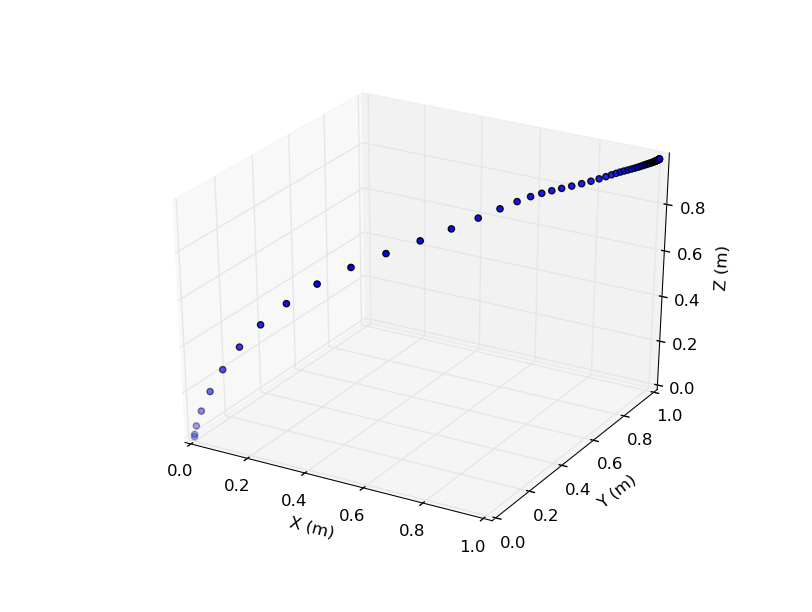
\includegraphics[width=\textwidth]{Figures/typical_run_time_3D_path.png}
		\rule{35em}{0.5pt}
	\caption[typical run 3D path]{A typical run - the 3D path}
	\label{fig:typical run 3D path}
\end{figure}

\begin{figure}[htbp]
	\centering
		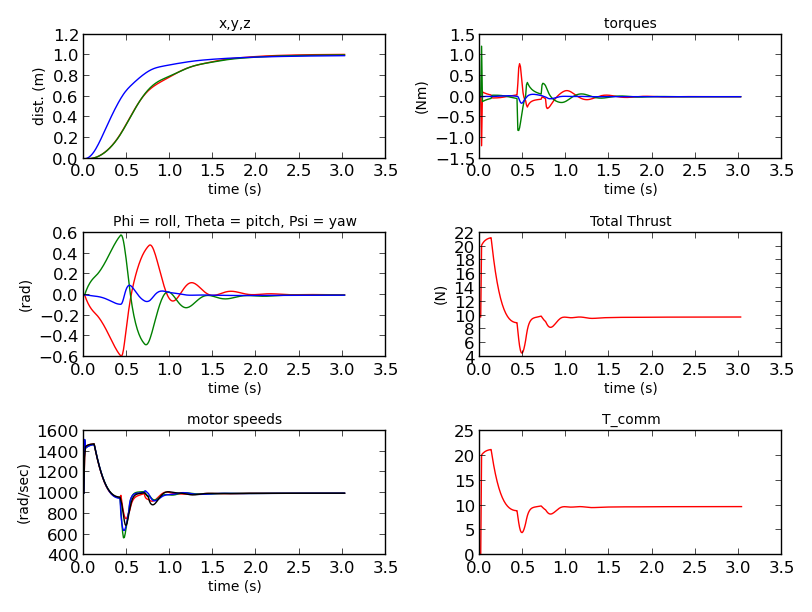
\includegraphics[width=\textwidth]{Figures/typical_run_time_domain.png}
		\rule{35em}{0.5pt}
	\caption[typical run time domain]{A typical run - time domain}
	\label{fig:typical run time domain}
\end{figure}


\begin{table}\label{table:params}
\begin{doublespace}
\centering
\begin{tabular}{l l l}
    Simulation Parameters\\
    \hline
    $g = -9.81            $& $ \frac{m}{s^2}          $ & acceleration due to gravity\\
    $m = 1                $& $ kg                      $ & mass\\ 
    $L = 1                $& $ m                       $ & length of quadrotor arm\\
    $b = 10^{-6}          $& $ \frac{N m s^2}{Rad^2}  $ & aerodynamic torque coefficient\\
    $k = 2.45*10^{-6}     $& $ \frac{N s^2}{Rad^2}    $ & aerodynamic thrust coefficient\\
    $Ixx = 5.0*10^{-3}    $& $ \frac{N m s^2}{Rad}    $ & moments of inertia \\
    $Iyy = 5.0*10^{-3}    $& $ \frac{N m s^2}{Rad}    $ & \\
    $Izz = 10.0*10^{-3}   $& $ \frac{N m s^2}{Rad}    $ & \\
    \hline
\end{tabular}
\caption[Simulation Parameters]{Simulation Parameters}
\end{doublespace}
\end{table}

\begin{figure}[htbp]
	\centering
		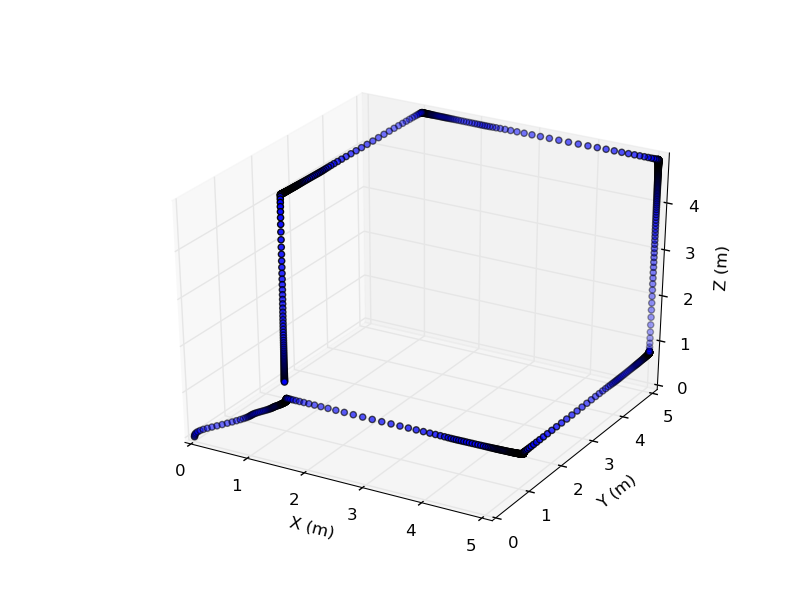
\includegraphics[width=\textwidth]{Figures/CubeEdges3D.png}
		\rule{35em}{0.5pt}
	\caption[Cube Edges]{Tracing some of the edges of a 4m cube - the 3D path}
	\label{fig:Cube Edges 3D}
\end{figure}

\begin{figure}[htbp]
	\centering
		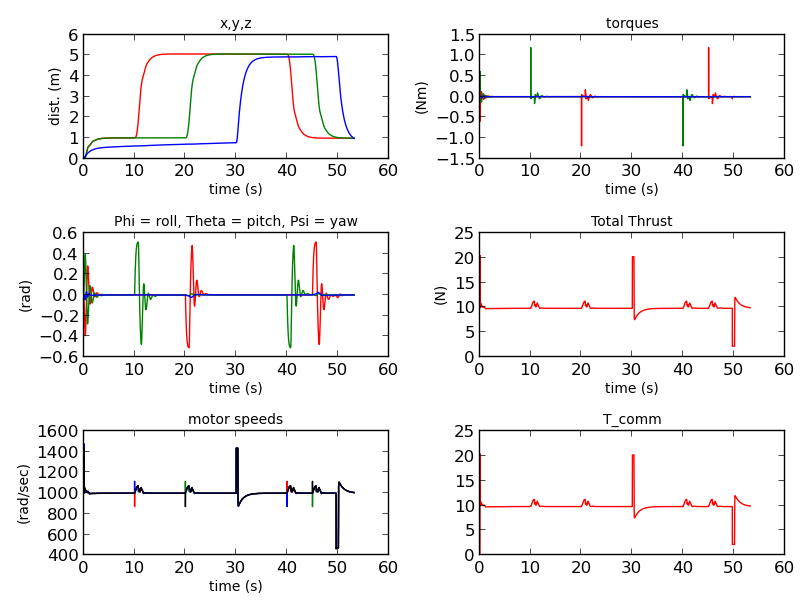
\includegraphics[width=\textwidth]{Figures/CubeEdgesGraphs.png}
		\rule{35em}{0.5pt}
	\caption[Cube Edges]{Tracing some of the edges of a 4m cube - time domain plots}
	\label{fig:Cube Edges Time Domain}
\end{figure}


\begin{figure}[htbp]
	\centering
		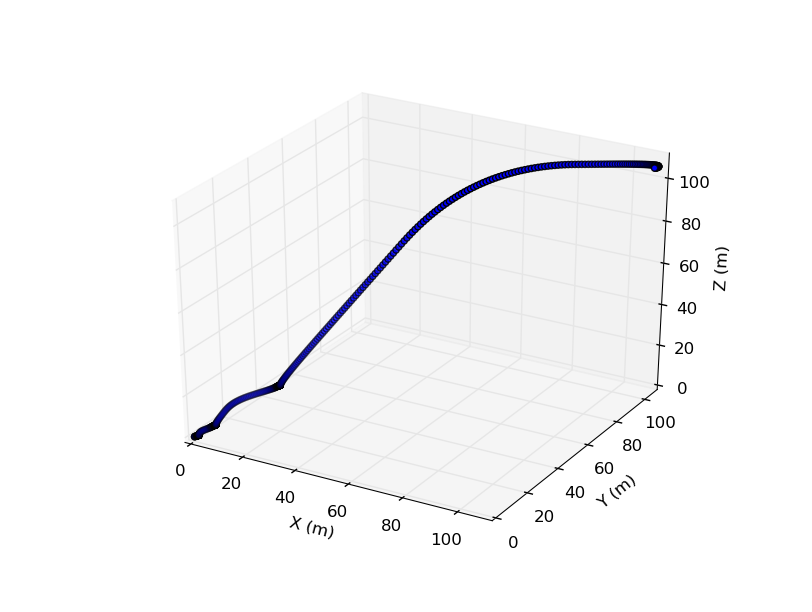
\includegraphics[width=\textwidth]{Figures/largeSetpointDifferencesTest_3d.png}
		\rule{35em}{0.5pt}
	\caption[largeSetpointDifferencesTest3D path]{Testing the control with larger set points - the 3D path}
	\label{fig:largeSetpointDifferencesTest3D path}
\end{figure}

\begin{figure}[htbp]
	\centering
		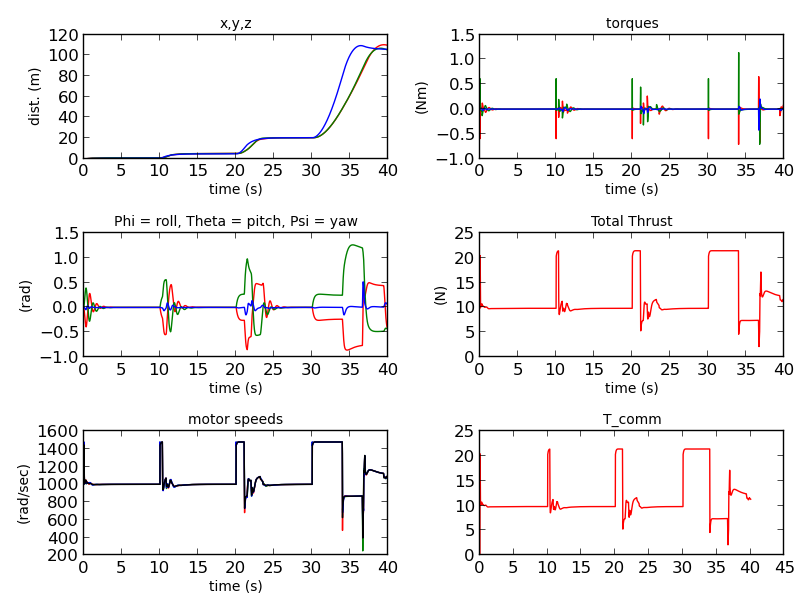
\includegraphics[width=\textwidth]{Figures/largeSetpointDifferencesTest_timedomain.png}
		\rule{35em}{0.5pt}
	\caption[largeSetpointDifferencesTesttimedomain]{Testing the control with larger set points - time domain plots }
	\label{fig:largeSetpointDifferencesTesttimedomain}
\end{figure}





